\documentclass[aspectratio=169]{beamer}

\usetheme{default}
\useoutertheme[subsection=false]{miniframes}
\usecolortheme{default}
\setbeamercolor{structure}{fg=black}

\usepackage{amsmath,amssymb}
\usepackage{mathtools}
\usepackage{booktabs}
\usepackage{tikz}
\usetikzlibrary{fit,calc,positioning,arrows.meta,backgrounds,shadows.blur,shapes.geometric,decorations.pathreplacing}
\usepackage{svg}
\usepackage{graphicx}
\usepackage{pifont} % \ding{51}/\ding{55} check and cross marks

% --- Talk colour palette (vivid) ---
\definecolor{palCitron}{HTML}{FFCA3A}   % vivid yellow
\definecolor{palOlivine}{HTML}{8AC926}  % vivid green
\definecolor{palCerulean}{HTML}{1982C4} % vivid blue
\definecolor{palGray}{HTML}{6A6F77}     % neutral slate grey
\definecolor{palCoral}{HTML}{FF595E}    % vivid coral / red

% --- Notation macros (copied from the paper preamble) ---
\newcommand{\psix}{\ensuremath{\mathrm{P4_{16}}}}
\newcommand{\pfour}{\ensuremath{\mathrm{P4_{14}}}}

% Temporal-logic and verification notation.
\newcommand{\CTL}{\ensuremath{\mathrm{CTL}}}
\newcommand{\LTL}{\ensuremath{\mathrm{LTL}}}
\newcommand{\CTLstar}{\ensuremath{\mathrm{CTL}^{*}}}
\newcommand{\AP}{\ensuremath{\mathit{AP}}}
\newcommand{\True}{\ensuremath{\mathsf{true}}}
\newcommand{\Next}{\ensuremath{\mathop{\mathbf{X}}}}
\newcommand{\Until}{\ensuremath{\mathbin{\mathbf{U}}}}
\newcommand{\WeakUntil}{\ensuremath{\mathbin{\mathbf{W}}}}
\newcommand{\Globally}{\ensuremath{\mathop{\mathbf{G}}}}
\newcommand{\Eventually}{\ensuremath{\mathop{\mathbf{F}}}}
\newcommand{\AllPaths}{\ensuremath{\forall}}
\newcommand{\SomePath}{\ensuremath{\exists}}
\newcommand{\AX}[1]{\ensuremath{\AllPaths\,\Next\,#1}}
\newcommand{\EX}[1]{\ensuremath{\SomePath\,\Next\,#1}}
\newcommand{\AG}[1]{\ensuremath{\AllPaths\,\Globally\,#1}}
\newcommand{\EG}[1]{\ensuremath{\SomePath\,\Globally\,#1}}
\newcommand{\AF}[1]{\ensuremath{\AllPaths\,\Eventually\,#1}}
\newcommand{\EF}[1]{\ensuremath{\SomePath\,\Eventually\,#1}}
\newcommand{\AU}[2]{\ensuremath{\AllPaths[#1 \Until #2]}}
\newcommand{\EU}[2]{\ensuremath{\SomePath[#1 \Until #2]}}

% Specification-language notation (copied from the paper preamble).
\newcommand{\specExpr}{\ensuremath{e}}
\newcommand{\specBlock}{\ensuremath{q}}
\newcommand{\specLoc}{\ensuremath{\mathit{loc}}}
\newcommand{\specAtom}{\ensuremath{\mathit{atom}}}
\newcommand{\specHit}{\ensuremath{\mathit{hit}}}
\newcommand{\specDrop}{\ensuremath{\mathit{drop}}}
\newcommand{\specBegin}{\ensuremath{\mathsf{begin}}}
\newcommand{\specEnd}{\ensuremath{\mathsf{end}}}
\newcommand{\ltlFormula}{\ensuremath{\varphi}}

\usepackage[style=numeric,backend=biber]{biblatex}
\addbibresource{references.bib}

% Keep the appendix (references) slides out of the total frame count.
\usepackage{appendixnumberbeamer}

% --- Footnote citation command (copied from the ICTopen2026 deck) ---
\newbibmacro*{authorurlcite:body}{%
  \printnames{author}%
  \setunit{\addperiod\space}%
  \iffieldundef{url}
    {\printfield[citetitle]{title}}
    {\href{\thefield{url}}{\printfield[citetitle]{title}}}%
  \iffieldundef{year}
    {}
    {\setunit{\addperiod\space}\printfield{year}}%
  \iffieldundef{doi}
    {\iffieldundef{url}
       {}
       {\setunit{\addperiod\space}URL:\space\href{\thefield{url}}{\nolinkurl{\thefield{url}}}}}
    {\setunit{\addperiod\space}DOI:\space\href{https://doi.org/\thefield{doi}}{\nolinkurl{\thefield{doi}}}}%
}

\DeclareCiteCommand{\footauthorurlcite}[\mkbibfootnote]
  {\usebibmacro{prenote}}
  {\usebibmacro{authorurlcite:body}}
  {\multicitedelim}
  {\usebibmacro{postnote}}

\setbeamertemplate{navigation symbols}{}

% lhs2TeX preamble (provides hscode environment, polytable, etc.)
\let\Bbbk\relax
\input{hs/pre.tex}

% Overlay-safe token highlight for lhs2TeX/polytable output. Avoid TikZ nodes
% here: they corrupt polytable's alignment state when the hscode block closes.
\newcommand{\anchornode}[2]{%
  \alt<2->{\textcolor{red}{\ensuremath{#2}}}{\ensuremath{#2}}}

\setbeamertemplate{headline}{}

\usepackage[T1]{fontenc}
\usepackage{zi4} % Inconsolata monospace font
\usepackage{helvet} % Helvetica for sans-serif

% Footline configuration with logos
\setbeamertemplate{footline}{%
  \begin{beamercolorbox}[wd=\paperwidth,ht=3ex,dp=1.5ex,leftskip=2ex,rightskip=2ex]{page number in head/foot}%
    \raisebox{-0.1cm}{\includegraphics[height=0.45cm]{uvalogo_tag_p.eps}}%
    \hspace{0.05cm}%
    \includegraphics[height=0.35cm]{smallLogo.pdf}%
    \hfill%
    \insertframenumber{} / \inserttotalframenumber%
  \end{beamercolorbox}%
}


\title{P4Check}
\subtitle{A Practical Verification Framework for Stateful P4 Data Planes}
\author{Tommaso Pacciani}
\institute{Informatics Institute, University of Amsterdam}
\date{\today}

\begin{document}

\begin{frame}[plain]
  \centering
  \vspace{\fill}
  {\usebeamerfont{title}\usebeamercolor[fg]{title}\inserttitle\par}
  \vspace{0.4em}
  {\usebeamerfont{subtitle}\usebeamercolor[fg]{subtitle}\insertsubtitle\par}
  \vspace{1.6em}
  {\large Tommaso Pacciani\par}
  \vspace{0.4em}
  {\small Supervisors: L.\ Thomas van Binsbergen, Chrysa Papagianni\par}
  \vspace{0.9em}
  {\small\insertinstitute\par}
  \vspace{0.4em}
  {\small\insertdate\par}
  \vspace{\fill}
  \makebox[\linewidth][c]{%
    \raisebox{-0.5\height}{\includegraphics[height=1.2cm]{mns_logo1.png}}%
    \hspace{2cm}%
    \raisebox{-0.5\height}{\includesvg[height=1.8cm]{fns_logo.svg}}%
  }
  \vspace{1em}
\end{frame}

\begin{frame}{Why Formal Methods?}
  % Flow for the speaker:
  %  (1) Dijkstra quote sets the frame, testing samples, it never proves absence.
  %  (2) Physical analogy, a proof is bounded by its model (bridge load vs. a ship
  %      striking a pier). Swap in a traffic light or an N-k power grid if preferred.
  %  (3) Same idea in code, tools prove safety and functional specs, but only
  %      relative to a model (correct compiler, correct hardware, faithful spec).
  %  (4) Takeaway, verification reasons over every input at once, stronger than any
  %      test suite, yet blind past the model. Testing still covers the real world.

  % Dijkstra quote
  \onslide<1->{%
  \vspace{0.15cm}
  \begin{quote}
    \large\itshape
    ``Program testing can be used to show the presence of bugs,\\
    but never to show their absence.''
    \begin{flushright}
      \normalfont\normalsize\textcolor{palGray}{Edsger W. Dijkstra, 1969}
    \end{flushright}
  \end{quote}}

  \vspace{0.3em}

  \begin{columns}[T,onlytextwidth]
    \begin{column}{0.48\textwidth}
      \begin{block}<2->{}
        \small
        \begin{itemize}
          \item A test samples real-world behavior for some specific inputs.
          \item Formal methods can give proofs for all possible inputs.
        \end{itemize}
        \par\vspace{0.45em}
      \end{block}
    \end{column}

    \begin{column}{0.48\textwidth}
      \begin{block}<3->{}
        \small
        \itshape ``All models are wrong, but some are useful.''
        \hfill \normalfont\textcolor{palGray}{George Box}
        \par\vspace{0.5em}
        For example, analyzing a C program to prove its correctness does not provide guarantees about the faithfulness of the compiler.
      \end{block}
    \end{column}
  \end{columns}

  \vspace{0.2em}

  % takeaway banner
  \onslide<4->{%
  \begin{center}
    \setlength\fboxsep{9pt}
    \colorbox{palCoral!12}{%
      \begin{minipage}{0.9\textwidth}\small
        \centering
        For P4 specifically, the input space of a program is generally large, programs are not modularly testable, and a program is written for a specific target, so testing it requires physical hardware. This work provides an alternative to testing by formally modeling P4, letting you reason about (parts of a) program.
      \end{minipage}}
  \end{center}}
\end{frame}

\begin{frame}{P4Check}
  \begin{columns}[T,onlytextwidth]

    % Left: identity / what it is
    \begin{column}{0.5\textwidth}
      A formalization of P4 in Haskell by means of a definitional interpreter
        \begin{itemize}\setlength\itemsep{8pt}
        \item \textbf{Verification}: Powered by \textbf{symbolic execution} and bounded
              \textbf{model checking}.
        \item Broad \psix{} coverage, of the core language and
              \textbf{architectures}.
      \end{itemize}
    \end{column}

    % Right: capabilities
    \begin{column}{0.46\textwidth}
      \begin{block}{Capabilities}
        \small
        \begin{itemize}\setlength\itemsep{6pt}
          \item[\textcolor{palOlivine!60!black}{\checkmark}]
                \textbf{Correctness Properties} % TODO needs example
                Single-packet assertions and multi-packet, stateful behavior
                written as temporal (\LTL{}) properties.
          \item[\textcolor{palOlivine!60!black}{\checkmark}]
                \textbf{Step through \emph{why} it fails.}
                A back-in-time debugger replays counterexamples, so you can explore the
                execution that led to a violation.
        \end{itemize}
      \end{block}
    \end{column}

  \end{columns}
\end{frame}

% \begin{frame}{Colour Palette Preview}
%   \centering
%   \vspace{0.4em}
%   \begin{tikzpicture}[
%       swatch/.style={rounded corners=4pt, minimum width=2.4cm, minimum height=2.4cm},
%       lbl/.style={font=\footnotesize\sffamily, align=center}
%     ]
%     \foreach \col/\hex/\name [count=\i from 0] in {%
%         palCitron/FFCA3A/Citron,
%         palOlivine/8AC926/Olivine,
%         palCerulean/1982C4/Cerulean,
%         palGray/6A6F77/Grey,
%         palCoral/FF595E/Coral} {
%       \node[swatch, fill=\col] (s\i) at (\i*2.7,0) {};
%       \node[lbl, below=4pt of s\i] {\name\\\texttt{\#\hex}};
%     }
%   \end{tikzpicture}

%   \vspace{1.2em}

%   % Sample usage so you can judge text/accents against the palette
%   \begin{tikzpicture}[font=\sffamily]
%     \node[rounded corners=4pt, fill=palCerulean, text=white,
%           inner sep=6pt, font=\bfseries] (a) at (0,0) {Heading / accent};
%     \node[rounded corners=4pt, draw=palOlivine, line width=1.2pt,
%           text=palOlivine!60!black, inner sep=6pt, right=6pt of a] (b) {Outlined box};
%     \node[rounded corners=4pt, fill=palCitron, text=black,
%           inner sep=6pt, right=6pt of b] (c) {Highlight};
%     \node[rounded corners=4pt, fill=palCoral, text=white,
%           inner sep=6pt, right=6pt of c] (d) {Emphasis};
%     \node[text=palGray, right=10pt of d] {body text in grey};
%   \end{tikzpicture}
% \end{frame}

% \begin{frame}{Index}
%   \begin{tikzpicture}[remember picture, overlay]
%     \node at (current page.center) {\resizebox{0.9\paperwidth}{!}{\insertnavigation{\paperwidth}}};
%   \end{tikzpicture}
% \end{frame}

\section{State of the art}
% Speaker notes:
% This slide has multiple goals one goal is to end with the bridge to debugging to motivate our work. somethign like Cruicially: only the private tool Aquila explores the process after a property is violated
% another goal is to introduce undefined behavior and bridge that to we can detect these automically. For corencresntss a user might want define corectness properties. can be thought of like tets. invaruiant on their program. . can for example be used in a devops pipeline (exactly like tests.) . 
% Concurrency point (from the paper's related work): HOL4P4 is the one
%   formalization that actually models P4's concurrency. Its operational
%   semantics captures the concurrency model and lets you reason about thread
%   interleavings and data races. None of the automated tools on this axis do
%   that; they reason about a single packet in isolation.
% Aquila / debugging point (the bridge to our work): Aquila is the only tool
%   here that does anything past a yes/no answer. After a property fails it can
%   localize which parts of the program caused the failure. It does this by
%   punching a hole in a candidate region and trying to synthesize a
%   replacement that makes the property hold again. If it can, that region was
%   to blame. This is the closest existing work to root-cause diagnosis, but it
%   is a private tool and it is quite different from a step-by-step debugger,
%   which is the gap we fill.
% Draft notes for the landscape slide (kept as comments; not typeset):
% Verification Tools -> Properties: static safety (reading an invalid header,
%   accessing a register/array index out of bounds, reading possibly
%   undefined behaviour).
% Formalizations of P4:
%   - language workbenches & metalanguages: K framework, P4 SpecTec
%   - theorem provers: HOL4P4 (models concurrency: thread interleavings, races)

\begin{frame}{P4 Formal Methods Landscape}
  \vspace{-0.2em}
  \centering
  \scalebox{0.86}{%
  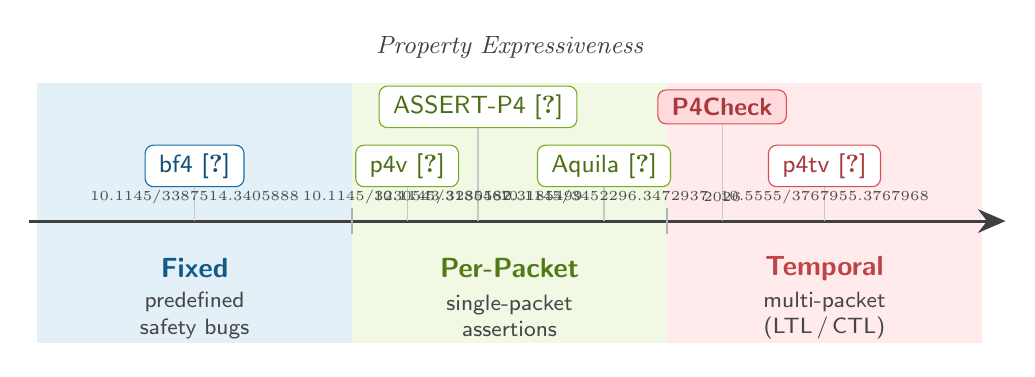
\begin{tikzpicture}[
      tool/.style={rounded corners=3pt, draw, fill=white, font=\small\sffamily,
                   inner xsep=5pt, inner ysep=3pt},
      fx/.style={tool, draw=palCerulean!85!black, text=palCerulean!60!black},
      pp/.style={tool, draw=palOlivine!85!black,  text=palOlivine!55!black},
      tp/.style={tool, draw=palCoral!85!black,    text=palCoral!65!black},
      zone/.style={font=\normalsize\bfseries\sffamily},
      gloss/.style={font=\footnotesize\sffamily, text=gray!55!black, align=center}
    ]
    % faint background band per region of the axis
    \begin{scope}[on background layer]
      \fill[palCerulean!12] (0,-1.55) rectangle (4,1.75);
      \fill[palOlivine!12]  (4,-1.55) rectangle (8,1.75);
      \fill[palCoral!12]    (8,-1.55) rectangle (12,1.75);
    \end{scope}

    % name of the axis
    \node[font=\small\itshape, text=gray!50!black] at (6,2.2) {Property Expressiveness};

    % the single axis arrow
    \draw[-{Stealth[length=3.5mm,width=3mm]}, line width=1.1pt, black!75] (-0.1,0) -- (12.3,0);
    \coordinate (O) at (0,0);
    % faint region separators
    \foreach \x in {4,8}{\draw[black!30] (\x,-0.16) -- (\x,0.16);}

    % region labels + one-line glosses, under the arrow
    \node[zone, text=palCerulean!70!black] at (2,-0.6)   {Fixed};
    \node[zone, text=palOlivine!60!black]  at (6,-0.6)   {Per-Packet};
    \node[zone, text=palCoral!75!black]    at (10,-0.6)  {Temporal};
    \node[gloss] at (2,-1.2)  {predefined\\safety bugs};
    \node[gloss] at (6,-1.2)  {single-packet\\assertions};
    \node[gloss] at (10,-1.2) {multi-packet\\(LTL\,/\,CTL)};

    % tools placed on the axis at their expressiveness position,
    % revealed progressively: bf4, then the per-packet group, then p4tv.
    % within the per-packet bucket tools are ordered left to right by year:
    % p4v (2018), ASSERT-P4 (2018), Aquila (2021).
    \node<1->[fx] (bf4)  at (2,0.7)    {bf4~\cite{10.1145/3387514.3405888}};
    \node<2->[pp] (p4v)  at (4.7,0.7)  {p4v~\cite{10.1145/3230543.3230582}};
    \node<2->[pp] (as)   at (5.6,1.45) {ASSERT-P4~\cite{10.1145/3185467.3185499}};
    \node<2->[pp] (aq)   at (7.2,0.7)  {Aquila~\cite{10.1145/3452296.3472937}};
    \node<3->[tp] (p4tv) at (10,0.7)   {p4tv~\cite{10.5555/3767955.3767968}};
    % P4Check (ours): placed less expressive than p4tv, revealed after the
    % "subset" bullet. Year hardcoded (no bib entry yet).
    \node<5->[tp, fill=palCoral!22, font=\small\sffamily\bfseries] (p4c) at (8.7,1.45) {P4Check};

    % subtle stems tying each tool to its point on the axis
    % (each stem appears together with its tool)
    \draw<1->[black!22, thin] (bf4.south)   -- (bf4.south   |- O);
    \draw<2->[black!22, thin] (p4v.south)   -- (p4v.south   |- O);
    \draw<2->[black!22, thin] (aq.south)    -- (aq.south    |- O);
    \draw<2->[black!22, thin] (as.south)    -- (as.south    |- O);
    \draw<3->[black!22, thin] (p4tv.south)  -- (p4tv.south  |- O);
    \draw<5->[black!22, thin] (p4c.south)   -- (p4c.south   |- O);

    % year of publication, pulled from the bib entry (\citeyear), next to
    % each tool's point on the axis
    \node<1->[font=\tiny, text=gray!60!black] at (2,0.30)   {\citeyear{10.1145/3387514.3405888}};
    \node<2->[font=\tiny, text=gray!60!black] at (4.7,0.30) {\citeyear{10.1145/3230543.3230582}};
    \node<2->[font=\tiny, text=gray!60!black] at (5.6,0.30) {\citeyear{10.1145/3185467.3185499}};
    \node<2->[font=\tiny, text=gray!60!black] at (7.2,0.30) {\citeyear{10.1145/3452296.3472937}};
    \node<3->[font=\tiny, text=gray!60!black] at (10,0.30)  {\citeyear{10.5555/3767955.3767968}};
    \node<5->[font=\tiny, text=gray!60!black] at (8.7,0.30) {2026};
  \end{tikzpicture}}

  \vspace{0.4em}
  \begin{itemize}\small\setlength\itemsep{0.35em}
    \item<4-> These tools cover only a subset of the core P4 language.
    \item<6-> Theorem provers (HOL4P4~\cite{hol4p4,10.1145/3565475.3569081,10.1007/978-3-031-86695-1_5},
              Verifiable P4~\cite{10.4230/LIPIcs.ITP.2023.32}): cover the full language,
              even concurrency, but proofs are by hand or per packet.
    \item<7-> Language workbenches and metalanguages
              (P4 SpecTec, P4K~\cite{kheradmand2018p4kformalsemanticsp4})
              give executable specifications of P4.
    \item<8-> \textcolor{palCoral!75!black}{\textbf{None of them, automated or interactive,
              offer a step-by-step debugger for failures.}}
  \end{itemize}

  \vfill
\end{frame}

\section{Background}

\input{background.tex}


\section{Implementation}
% Combined slide: the architecture diagram on top, the flow in two columns
% below it, and a progress-marker overlay (step 2) highlighting the Frontend +
% Static Semantics (interpreter) part. The overlay hook in p4checkarch.tikz
% lets us highlight without duplicating the figure source.
\begin{frame}{Architecture and Flow}
\centering
\resizebox{!}{0.52\textheight}{%
  \begingroup
  \def\PFourArchOverlay{%
    \only<2->{%
      \draw[palCoral, line width=1.6pt, rounded corners=6pt]
        ([xshift=-0.25cm, yshift=0.20cm]frontend.north west)
        rectangle
        ([xshift=0.25cm, yshift=-0.12cm]staticsem.south east);
    }%
  }%
  \begingroup%
% Canonical geometry for this figure. Keep these definitions local so callers
% cannot accidentally change the rendered aspect ratio before inputting it.
\def\PFourArchBoxXSep{0.08cm}%
\def\PFourInstrumentBelowFrontend{0.65cm}%
\def\PFourToolStageWidth{1.58cm}%
\def\PFourVerifyAfterInstrument{0.5cm}%
\def\PFourLocalizeBelowCounterexample{0.75cm}%
\def\PFourVerifyResultXSep{0.40cm}%
\def\PFourResultArtifactXSep{0.75cm}%
\def\PFourOutputArtifactXSep{0.25cm}%
\def\PFourArchBoxYSep{0.08cm}%
\def\PFourSymbolicBandPad{0.08cm}%
% Fonts: use the deck's default font (no biolinum), keep zi4 for monospace.
\def\PFourArchText{\fontsize{6}{7}\selectfont}%
\def\PFourArchTiny{\fontsize{5}{6}\selectfont}%
\def\PFourArchMonoTiny{\fontencoding{T1}\fontfamily{zi4}\fontsize{5}{6}\selectfont}%
\def\PFourArchLarge{\fontsize{10}{12}\selectfont}%
\begin{tikzpicture}[
    font=\PFourArchText,
    >=Latex,
    box/.style={
        rectangle,
        draw=black!70,
        fill=white,
        align=center,
        minimum height=0.72cm,
        inner xsep=4pt,
        inner ysep=3pt
    },
    inputbox/.style={
        ellipse,
        draw=black!70,
        fill=palOlivine!25,
        align=center,
        minimum width=1.45cm,
        minimum height=0.58cm,
        inner xsep=4pt,
        inner ysep=2pt
    },
    stage/.style={
        box,
        fill=palGray!12,
        minimum width=1.20cm
    },
    toolstage/.style={
        stage,
        minimum width=\PFourToolStageWidth,
        text width=1.28cm,
        align=center
    },
    artifact/.style={
        ellipse,
        draw=black!70,
        fill=palCoral!22,
        align=center,
        minimum width=1.35cm,
        minimum height=0.58cm,
        inner xsep=4pt,
        inner ysep=2pt
    },
    compactartifact/.style={
        artifact,
        font=\PFourArchTiny,
        minimum width=1.30cm,
        minimum height=0.50cm,
        inner xsep=2.5pt,
        inner ysep=1.5pt
    },
    widebox/.style={
        box,
        fill=palGray!7,
        minimum width=2.86cm
    },
    semblock/.style={
        box,
        fill=white,
        font=\PFourArchTiny,
        minimum width=0.93cm,
        minimum height=0.48cm,
        inner xsep=3pt,
        inner ysep=2pt
    },
    note/.style={
        font=\PFourArchText\bfseries,
        align=center
    },
    arrow/.style={
        -{Latex[length=2mm]},
        line width=0.45pt,
        shorten >=1pt,
        shorten <=1pt
    },
    dataarrow/.style={
        arrow,
        dashed,
        draw=black!65
    },
    semarrow/.style={
        -{Latex[length=1.4mm]},
        line width=0.35pt,
        shorten >=1pt,
        shorten <=1pt
    }
]

% Inputs.
\node[inputbox] (source) at (0,2.85) {P4 Source\\Code};

% Frontend.
\node[box, minimum width=1.55cm, minimum height=2.10cm, fill=palGray!9, anchor=north]
    (frontend) at (2.0,3.575) {};
\node[note, anchor=north] at (frontend.north) {Frontend};
\node[stage] (parser) at (2.0,2.86) {Parser};
\node[stage] (ast) at (2.0,1.96) {AST};
\node[toolstage, anchor=north] (instrument)
    at ([yshift=-\PFourInstrumentBelowFrontend]frontend.south) {Instrument};
\node[inputbox] (property) at (source.center |- instrument.center) {Property};

% Haskell implementation.
\node[widebox, minimum height=1.48cm]
    (interpreter) at (4.65,2.77) {};
\node[note, anchor=north] (interp-title) at (interpreter.north) {Interpreter};
\path[fill=palCitron, opacity=0.55]
    let \p1 = (interpreter.south west) in
    (\x1,\y1) rectangle (9.48cm,3.52cm);
\path let \p1 = (interpreter.south west) in
    node[note, anchor=south, yshift=0.05cm]
    at ($(\x1,3.52cm)!0.5!(9.48cm,3.52cm)$) {Concrete mode (Debugging)};
\node[font=\PFourArchTiny, align=center] at ([yshift=0.08cm]interpreter.center)
    {Unified: Concrete \& Symbolic};
\node[semblock] (staticsem) at ([xshift=-0.58cm,yshift=-0.42cm]interpreter.center)
    {Static\\Semantics};
\node[semblock] (dynamicsem) at ([xshift=0.58cm,yshift=-0.42cm]interpreter.center)
    {Dynamic\\Semantics};
\draw[semarrow] (staticsem.east) -- (dynamicsem.west);

% Concrete/debugging outputs.
\node[box, minimum width=1.22cm, minimum height=0.96cm, inner sep=0pt]
    (debugger) at (8.65,2.77) {};
\node[compactartifact, minimum width=0.82cm, minimum height=0.42cm,
    inner xsep=2pt, inner ysep=1pt]
    (trace) at ($(interpreter.east)!0.5!(debugger.west)$) {Trace};
\path[fill=palGray!22, draw=black!65, line width=0.22pt]
    ([xshift=-0.61cm,yshift=0.34cm]debugger.center)
    rectangle ++(1.22cm,0.14cm);
\fill[palCoral!80!black]
    ([xshift=-0.53cm,yshift=0.41cm]debugger.center) circle (0.018cm);
\node[font=\PFourArchMonoTiny, anchor=east]
    at ([xshift=0.54cm,yshift=0.41cm]debugger.center) {\textless\ \textgreater};
\draw[line width=0.18pt, draw=black!40]
    ([xshift=-0.34cm,yshift=0.30cm]debugger.center) -- ++(0,-0.55cm);
\fill[palCitron]
    ([xshift=-0.30cm,yshift=0.12cm]debugger.center)
    rectangle ++(0.80cm,0.12cm);
\node[font=\PFourArchMonoTiny, text=black!50, anchor=west]
    at ([xshift=-0.47cm,yshift=0.18cm]debugger.center) {1};
\node[font=\PFourArchMonoTiny, text=black!50, anchor=west]
    at ([xshift=-0.47cm,yshift=0.05cm]debugger.center) {2};
\node[font=\PFourArchMonoTiny, text=black!50, anchor=west]
    at ([xshift=-0.47cm,yshift=-0.08cm]debugger.center) {3};
\node[font=\PFourArchMonoTiny, text=black!50, anchor=west]
    at ([xshift=-0.47cm,yshift=-0.21cm]debugger.center) {4};
\node[font=\PFourArchMonoTiny, anchor=west]
    at ([xshift=-0.24cm,yshift=0.18cm]debugger.center) {if(hit)};
\node[font=\PFourArchMonoTiny, anchor=west]
    at ([xshift=-0.14cm,yshift=0.05cm]debugger.center) {apply};
\node[font=\PFourArchMonoTiny, anchor=west]
    at ([xshift=-0.24cm,yshift=-0.08cm]debugger.center) {else};
\node[font=\PFourArchMonoTiny, anchor=west]
    at ([xshift=-0.14cm,yshift=-0.21cm]debugger.center) {drop};
\fill[palCoral!80!black]
    ([xshift=-0.52cm,yshift=0.18cm]debugger.center) circle (0.026cm);
\draw[line width=0.22pt, draw=black!65]
    ([xshift=-0.61cm,yshift=-0.28cm]debugger.center) -- ++(1.22cm,0);
\node[font=\PFourArchMonoTiny, anchor=west]
    at ([xshift=-0.48cm,yshift=-0.38cm]debugger.center) {pkt};
\node[font=\PFourArchMonoTiny, anchor=west]
    at ([xshift=0.10cm,yshift=-0.38cm]debugger.center) {meta};
% Concrete mode label moved to yellow band path

% Symbolic/verification outputs.
\node[toolstage, anchor=west]
    (verify) at ([xshift=\PFourVerifyAfterInstrument,yshift=0.45cm]instrument.east) {Verify};
\node[font=\PFourArchLarge\bfseries, text=palOlivine!80!black, inner sep=1pt]
    (verifyok) at ([xshift=\PFourVerifyResultXSep,yshift=-0.28cm]verify.east) {\ding{51}};
\node[font=\PFourArchLarge\bfseries, text=palCitron!65!black, inner sep=1pt]
    (verifyunknown) at ([xshift=\PFourVerifyResultXSep]verify.east) {?};
\node[font=\PFourArchLarge\bfseries, text=palCoral!85!black, inner sep=1pt]
    (verifyfail) at ([xshift=\PFourVerifyResultXSep,yshift=0.28cm]verify.east) {\ding{55}};
\node[compactartifact, anchor=west]
    (counterexample) at ([xshift=\PFourResultArtifactXSep]verifyfail.east)
    {Counter-\\example};
\node[compactartifact, anchor=west]
    (propbreakpoint)
    at ([xshift=\PFourOutputArtifactXSep,yshift=-\PFourLocalizeBelowCounterexample]counterexample.east)
    {Breakpoint};
% Symbolic mode label moved to red band path

% Main flow.
\draw[arrow] (source.east) -- (parser.west);
\draw[arrow] (parser.south) -- (ast.north);
\draw[arrow] (ast.east) -- ++(0.30,0) |- (interpreter.west);
\draw[arrow] (interpreter.east) -- (trace.west);
\draw[arrow] (trace.east) -- (debugger.west);

% Instrumentation and verification flow.
\draw[dataarrow] (property.east) -- (instrument.west);
\draw[dataarrow] (frontend.south) -- (instrument.north);
\draw[dataarrow] (instrument.east) -- ++(0.26,0) -- ++(0,1.12) -| ([xshift=-1.0cm]interpreter.south);
\draw[dataarrow] ([xshift=0.35cm]interpreter.south) -- ++(0,-0.35) -| (verify.north);
\draw[dataarrow] (verify.east |- verifyfail.center) -- (verifyfail.west);
\draw[dataarrow] (verify.east |- verifyunknown.center) -- (verifyunknown.west);
\draw[dataarrow] (verify.east |- verifyok.center) -- (verifyok.west);
\draw[dataarrow] (verifyfail.east) -- (counterexample.west);
\draw[dataarrow] (property.south) -- ++(0,-0.5) -| ([xshift=-0.28cm]propbreakpoint.south);
\draw[dataarrow] (counterexample.north) -- ++(0,0.30)
    -| ([xshift=1.05cm]interpreter.south);
\draw[dataarrow] (propbreakpoint.north) --
    (propbreakpoint.north |- debugger.south);

\begin{scope}[on background layer]
    \path[fill=palCerulean!90, opacity=0.22]
        let
            \p1 = (interpreter.west),
            \p2 = ([yshift=-\PFourSymbolicBandPad]propbreakpoint.south),
            \p3 = ([yshift=\PFourSymbolicBandPad]counterexample.north)
        in
            (\x1,\y2) rectangle (9.48cm,\y3);
\end{scope}
% Place label below the red band using relative offset from its bottom edge
\path let
        \p1 = (interpreter.west),
        \p2 = ([yshift=-\PFourSymbolicBandPad]propbreakpoint.south)
    in
    node[note, anchor=north, yshift=-0.05cm]
    at ($(\x1,\y2)!0.5!(9.48cm,\y2)$) {Symbolic model (Verification)};

% Overlay hook: if the caller defined \PFourArchOverlay, execute it now.
% This lets progress-marker slides highlight parts of the diagram without
% duplicating the figure source.
\ifdefined\PFourArchOverlay\PFourArchOverlay\fi

\pgfresetboundingbox
\path[use as bounding box] (-0.90,-0.45) rectangle (9.70,3.95);

\end{tikzpicture}%
\endgroup%
%
  \endgroup
}

\vspace{0.6em}
\begin{columns}[T,onlytextwidth]
  \begin{column}{0.49\textwidth}
    \begin{itemize}\footnotesize\setlength\itemsep{2pt}
    \item Big-step semantics, dual concrete and symbolic execution using Grisette.
    \item For verification, instrumentation with ghost variables.
    \item Verification produces a counterexample, one or more packets.
    \end{itemize}
  \end{column}
  \begin{column}{0.49\textwidth}
    \begin{itemize}\footnotesize\setlength\itemsep{2pt}
    \item The counterexample can be fed to the concrete execution to obtain a small-step-like trace.
    \item The trace can be navigated with breakpoints.
    \end{itemize}
  \end{column}
\end{columns}
\end{frame}



% \section{Temporal verification}

% \begin{frame}{Three Levels of Properties}
% % TODO add examples
% \begin{columns}[T,onlytextwidth]
%   \begin{column}{0.54\textwidth}
%     \centering
%     \begin{tikzpicture}

%     \node[rectangle, rounded corners=6pt, draw=green!70!black, thick,
%           fill=green!8, minimum width=5.2cm, minimum height=2.0cm,
%           text=black, font=\scriptsize, align=left, inner sep=6pt] (L1) at (0, 2.4) {};
%     \node[anchor=north west, font=\bfseries\sffamily\small, text=green!60!black]
%       (L1T) at ([shift={(5pt,-4pt)}]L1.north west) {1. Intra-Packet};
%     \node[anchor=north west, font=\scriptsize, text width=4.6cm] at ([shift={(0,-2pt)}]L1T.south west)
%       {Properties about a \emph{single} packet's processing through one pipeline invocation.};

%     \node[rectangle, rounded corners=6pt, draw=orange!70!black, thick,
%           fill=orange!8, minimum width=5.2cm, minimum height=2.0cm,
%           text=black, font=\scriptsize, align=left, inner sep=6pt] (L2) at (0, 0) {};
%     \node[anchor=north west, font=\bfseries\sffamily\small, text=orange!60!black]
%       (L2T) at ([shift={(5pt,-4pt)}]L2.north west) {2. Inter-Packet (Stateful)};
%     \node[anchor=north west, font=\scriptsize, text width=4.6cm] at ([shift={(0,-2pt)}]L2T.south west)
%       {Properties relating the processing of \emph{multiple} packets via shared state (registers, counters, meters).};

%     \node[rectangle, rounded corners=6pt, draw=violet!70!black, thick,
%           fill=violet!8, minimum width=5.2cm, minimum height=2.0cm,
%           text=black, font=\scriptsize, align=left, inner sep=6pt] (L3) at (0, -2.4) {};
%     \node[anchor=north west, font=\bfseries\sffamily\small, text=violet!60!black]
%       (L3T) at ([shift={(5pt,-4pt)}]L3.north west) {3. Network-Wide};
%     \node[anchor=north west, font=\scriptsize, text width=4.6cm] at ([shift={(0,-2pt)}]L3T.south west)
%       {Properties spanning \emph{multiple switches} and the topology connecting them.};

%     \draw[->, thick, gray] ([xshift=2pt]L1.south east) -- ([xshift=2pt]L2.north east)
%       node[midway, right, font=\scriptsize\sffamily, text=gray] {+ state};
%     \draw[->, thick, gray] ([xshift=2pt]L2.south east) -- ([xshift=2pt]L3.north east)
%       node[midway, right, font=\scriptsize\sffamily, text=gray] {+ topology};

%     \end{tikzpicture}
%   \end{column}

%   \begin{column}{0.42\textwidth}
%   \end{column}
% \end{columns}
% \end{frame}

\begin{frame}{Architecture and Target Modeling}
  A P4 program with its architecture is an \textbf{under-specification}, leaving many behaviors implementation-defined. We model this as a three-level lattice to separate architecture-fixed facts from target-specific choices.

  \vspace{0.8em}
  \begin{block}{The Three-Level Target Lattice}
    \small
    \begin{itemize}\setlength\itemsep{4pt}
      \item \textbf{Level 0 (Language)}, the P4-16 standard over-approximation.
      \item \textbf{Level 1 (Architecture)}, narrows the language by what the specific architecture guarantees. For instance, v1model leaves register initialization free.
      \item \textbf{Level 2 (Target)}, a concrete device that fully pins the remaining choices. For example, bmv2 zero-initializes registers.
    \end{itemize}
  \end{block}
\end{frame}

\begin{frame}{Per-Construct Modeling Choices}
  \vspace{0.6em}
  \centering
  \begin{table}
    \centering
    \begin{tabular}{@{} l l @{}}
      \toprule
      \textbf{Construct} & \textbf{Modeling Approach} \\
      \midrule
      Packet & Size statically analyzed or $<$ MTU \\
      Parser & Fuel-bounded, error if exhausted \\
      Tables & Nondeterministic choice of action \\
      Recirculate & Fuel-bounded \\
      Register and Counter & Symbolic array, struct-of-arrays \\
      Meter & \emph{Not yet modeled} \\
      \multicolumn{2}{@{}l}{\textit{Checksum and Hash}} \\
      \quad \texttt{csum16}, \texttt{xor16}, \texttt{random} & Exact arithmetic, \texttt{random} fresh symbolic \\
      \quad \texttt{crc16}, \texttt{crc32}, custom CRCs & \emph{Over-approximation}, uninterpreted function \\
      \bottomrule
    \end{tabular}
  \end{table}
\end{frame}

% Progress-marker: highlight the Instrument + Symbolic verification region.
\begin{frame}{Architecture: Verification}
\centering
\resizebox{\linewidth}{!}{%
  \begingroup
  \def\PFourArchOverlay{%
    % Top-left uses Instrument's left edge but the top of the tallest element
    % in the region (Counterexample), so the box does not clip Verify, the
    % result marks, or the Counterexample ellipse.
    \draw[palCoral, line width=1.6pt, rounded corners=6pt]
      ($(instrument.west |- counterexample.north) + (-0.25cm, 0.20cm)$)
      rectangle
      ($(propbreakpoint.south east) + (0.25cm, -0.30cm)$);
  }%
  \begingroup%
% Canonical geometry for this figure. Keep these definitions local so callers
% cannot accidentally change the rendered aspect ratio before inputting it.
\def\PFourArchBoxXSep{0.08cm}%
\def\PFourInstrumentBelowFrontend{0.65cm}%
\def\PFourToolStageWidth{1.58cm}%
\def\PFourVerifyAfterInstrument{0.5cm}%
\def\PFourLocalizeBelowCounterexample{0.75cm}%
\def\PFourVerifyResultXSep{0.40cm}%
\def\PFourResultArtifactXSep{0.75cm}%
\def\PFourOutputArtifactXSep{0.25cm}%
\def\PFourArchBoxYSep{0.08cm}%
\def\PFourSymbolicBandPad{0.08cm}%
% Fonts: use the deck's default font (no biolinum), keep zi4 for monospace.
\def\PFourArchText{\fontsize{6}{7}\selectfont}%
\def\PFourArchTiny{\fontsize{5}{6}\selectfont}%
\def\PFourArchMonoTiny{\fontencoding{T1}\fontfamily{zi4}\fontsize{5}{6}\selectfont}%
\def\PFourArchLarge{\fontsize{10}{12}\selectfont}%
\begin{tikzpicture}[
    font=\PFourArchText,
    >=Latex,
    box/.style={
        rectangle,
        draw=black!70,
        fill=white,
        align=center,
        minimum height=0.72cm,
        inner xsep=4pt,
        inner ysep=3pt
    },
    inputbox/.style={
        ellipse,
        draw=black!70,
        fill=palOlivine!25,
        align=center,
        minimum width=1.45cm,
        minimum height=0.58cm,
        inner xsep=4pt,
        inner ysep=2pt
    },
    stage/.style={
        box,
        fill=palGray!12,
        minimum width=1.20cm
    },
    toolstage/.style={
        stage,
        minimum width=\PFourToolStageWidth,
        text width=1.28cm,
        align=center
    },
    artifact/.style={
        ellipse,
        draw=black!70,
        fill=palCoral!22,
        align=center,
        minimum width=1.35cm,
        minimum height=0.58cm,
        inner xsep=4pt,
        inner ysep=2pt
    },
    compactartifact/.style={
        artifact,
        font=\PFourArchTiny,
        minimum width=1.30cm,
        minimum height=0.50cm,
        inner xsep=2.5pt,
        inner ysep=1.5pt
    },
    widebox/.style={
        box,
        fill=palGray!7,
        minimum width=2.86cm
    },
    semblock/.style={
        box,
        fill=white,
        font=\PFourArchTiny,
        minimum width=0.93cm,
        minimum height=0.48cm,
        inner xsep=3pt,
        inner ysep=2pt
    },
    note/.style={
        font=\PFourArchText\bfseries,
        align=center
    },
    arrow/.style={
        -{Latex[length=2mm]},
        line width=0.45pt,
        shorten >=1pt,
        shorten <=1pt
    },
    dataarrow/.style={
        arrow,
        dashed,
        draw=black!65
    },
    semarrow/.style={
        -{Latex[length=1.4mm]},
        line width=0.35pt,
        shorten >=1pt,
        shorten <=1pt
    }
]

% Inputs.
\node[inputbox] (source) at (0,2.85) {P4 Source\\Code};

% Frontend.
\node[box, minimum width=1.55cm, minimum height=2.10cm, fill=palGray!9, anchor=north]
    (frontend) at (2.0,3.575) {};
\node[note, anchor=north] at (frontend.north) {Frontend};
\node[stage] (parser) at (2.0,2.86) {Parser};
\node[stage] (ast) at (2.0,1.96) {AST};
\node[toolstage, anchor=north] (instrument)
    at ([yshift=-\PFourInstrumentBelowFrontend]frontend.south) {Instrument};
\node[inputbox] (property) at (source.center |- instrument.center) {Property};

% Haskell implementation.
\node[widebox, minimum height=1.48cm]
    (interpreter) at (4.65,2.77) {};
\node[note, anchor=north] (interp-title) at (interpreter.north) {Interpreter};
\path[fill=palCitron, opacity=0.55]
    let \p1 = (interpreter.south west) in
    (\x1,\y1) rectangle (9.48cm,3.52cm);
\path let \p1 = (interpreter.south west) in
    node[note, anchor=south, yshift=0.05cm]
    at ($(\x1,3.52cm)!0.5!(9.48cm,3.52cm)$) {Concrete mode (Debugging)};
\node[font=\PFourArchTiny, align=center] at ([yshift=0.08cm]interpreter.center)
    {Unified: Concrete \& Symbolic};
\node[semblock] (staticsem) at ([xshift=-0.58cm,yshift=-0.42cm]interpreter.center)
    {Static\\Semantics};
\node[semblock] (dynamicsem) at ([xshift=0.58cm,yshift=-0.42cm]interpreter.center)
    {Dynamic\\Semantics};
\draw[semarrow] (staticsem.east) -- (dynamicsem.west);

% Concrete/debugging outputs.
\node[box, minimum width=1.22cm, minimum height=0.96cm, inner sep=0pt]
    (debugger) at (8.65,2.77) {};
\node[compactartifact, minimum width=0.82cm, minimum height=0.42cm,
    inner xsep=2pt, inner ysep=1pt]
    (trace) at ($(interpreter.east)!0.5!(debugger.west)$) {Trace};
\path[fill=palGray!22, draw=black!65, line width=0.22pt]
    ([xshift=-0.61cm,yshift=0.34cm]debugger.center)
    rectangle ++(1.22cm,0.14cm);
\fill[palCoral!80!black]
    ([xshift=-0.53cm,yshift=0.41cm]debugger.center) circle (0.018cm);
\node[font=\PFourArchMonoTiny, anchor=east]
    at ([xshift=0.54cm,yshift=0.41cm]debugger.center) {\textless\ \textgreater};
\draw[line width=0.18pt, draw=black!40]
    ([xshift=-0.34cm,yshift=0.30cm]debugger.center) -- ++(0,-0.55cm);
\fill[palCitron]
    ([xshift=-0.30cm,yshift=0.12cm]debugger.center)
    rectangle ++(0.80cm,0.12cm);
\node[font=\PFourArchMonoTiny, text=black!50, anchor=west]
    at ([xshift=-0.47cm,yshift=0.18cm]debugger.center) {1};
\node[font=\PFourArchMonoTiny, text=black!50, anchor=west]
    at ([xshift=-0.47cm,yshift=0.05cm]debugger.center) {2};
\node[font=\PFourArchMonoTiny, text=black!50, anchor=west]
    at ([xshift=-0.47cm,yshift=-0.08cm]debugger.center) {3};
\node[font=\PFourArchMonoTiny, text=black!50, anchor=west]
    at ([xshift=-0.47cm,yshift=-0.21cm]debugger.center) {4};
\node[font=\PFourArchMonoTiny, anchor=west]
    at ([xshift=-0.24cm,yshift=0.18cm]debugger.center) {if(hit)};
\node[font=\PFourArchMonoTiny, anchor=west]
    at ([xshift=-0.14cm,yshift=0.05cm]debugger.center) {apply};
\node[font=\PFourArchMonoTiny, anchor=west]
    at ([xshift=-0.24cm,yshift=-0.08cm]debugger.center) {else};
\node[font=\PFourArchMonoTiny, anchor=west]
    at ([xshift=-0.14cm,yshift=-0.21cm]debugger.center) {drop};
\fill[palCoral!80!black]
    ([xshift=-0.52cm,yshift=0.18cm]debugger.center) circle (0.026cm);
\draw[line width=0.22pt, draw=black!65]
    ([xshift=-0.61cm,yshift=-0.28cm]debugger.center) -- ++(1.22cm,0);
\node[font=\PFourArchMonoTiny, anchor=west]
    at ([xshift=-0.48cm,yshift=-0.38cm]debugger.center) {pkt};
\node[font=\PFourArchMonoTiny, anchor=west]
    at ([xshift=0.10cm,yshift=-0.38cm]debugger.center) {meta};
% Concrete mode label moved to yellow band path

% Symbolic/verification outputs.
\node[toolstage, anchor=west]
    (verify) at ([xshift=\PFourVerifyAfterInstrument,yshift=0.45cm]instrument.east) {Verify};
\node[font=\PFourArchLarge\bfseries, text=palOlivine!80!black, inner sep=1pt]
    (verifyok) at ([xshift=\PFourVerifyResultXSep,yshift=-0.28cm]verify.east) {\ding{51}};
\node[font=\PFourArchLarge\bfseries, text=palCitron!65!black, inner sep=1pt]
    (verifyunknown) at ([xshift=\PFourVerifyResultXSep]verify.east) {?};
\node[font=\PFourArchLarge\bfseries, text=palCoral!85!black, inner sep=1pt]
    (verifyfail) at ([xshift=\PFourVerifyResultXSep,yshift=0.28cm]verify.east) {\ding{55}};
\node[compactartifact, anchor=west]
    (counterexample) at ([xshift=\PFourResultArtifactXSep]verifyfail.east)
    {Counter-\\example};
\node[compactartifact, anchor=west]
    (propbreakpoint)
    at ([xshift=\PFourOutputArtifactXSep,yshift=-\PFourLocalizeBelowCounterexample]counterexample.east)
    {Breakpoint};
% Symbolic mode label moved to red band path

% Main flow.
\draw[arrow] (source.east) -- (parser.west);
\draw[arrow] (parser.south) -- (ast.north);
\draw[arrow] (ast.east) -- ++(0.30,0) |- (interpreter.west);
\draw[arrow] (interpreter.east) -- (trace.west);
\draw[arrow] (trace.east) -- (debugger.west);

% Instrumentation and verification flow.
\draw[dataarrow] (property.east) -- (instrument.west);
\draw[dataarrow] (frontend.south) -- (instrument.north);
\draw[dataarrow] (instrument.east) -- ++(0.26,0) -- ++(0,1.12) -| ([xshift=-1.0cm]interpreter.south);
\draw[dataarrow] ([xshift=0.35cm]interpreter.south) -- ++(0,-0.35) -| (verify.north);
\draw[dataarrow] (verify.east |- verifyfail.center) -- (verifyfail.west);
\draw[dataarrow] (verify.east |- verifyunknown.center) -- (verifyunknown.west);
\draw[dataarrow] (verify.east |- verifyok.center) -- (verifyok.west);
\draw[dataarrow] (verifyfail.east) -- (counterexample.west);
\draw[dataarrow] (property.south) -- ++(0,-0.5) -| ([xshift=-0.28cm]propbreakpoint.south);
\draw[dataarrow] (counterexample.north) -- ++(0,0.30)
    -| ([xshift=1.05cm]interpreter.south);
\draw[dataarrow] (propbreakpoint.north) --
    (propbreakpoint.north |- debugger.south);

\begin{scope}[on background layer]
    \path[fill=palCerulean!90, opacity=0.22]
        let
            \p1 = (interpreter.west),
            \p2 = ([yshift=-\PFourSymbolicBandPad]propbreakpoint.south),
            \p3 = ([yshift=\PFourSymbolicBandPad]counterexample.north)
        in
            (\x1,\y2) rectangle (9.48cm,\y3);
\end{scope}
% Place label below the red band using relative offset from its bottom edge
\path let
        \p1 = (interpreter.west),
        \p2 = ([yshift=-\PFourSymbolicBandPad]propbreakpoint.south)
    in
    node[note, anchor=north, yshift=-0.05cm]
    at ($(\x1,\y2)!0.5!(9.48cm,\y2)$) {Symbolic model (Verification)};

% Overlay hook: if the caller defined \PFourArchOverlay, execute it now.
% This lets progress-marker slides highlight parts of the diagram without
% duplicating the figure source.
\ifdefined\PFourArchOverlay\PFourArchOverlay\fi

\pgfresetboundingbox
\path[use as bounding box] (-0.90,-0.45) rectangle (9.70,3.95);

\end{tikzpicture}%
\endgroup%
%
  \endgroup
}
\end{frame}



\begin{frame}{Modeling the Control Plane}
  \vspace{0.3em}
  \begin{itemize}\small
    \item We abstract tables as one symbolic action choice.
  \end{itemize}
  \centering
  \vspace{0.3em}

  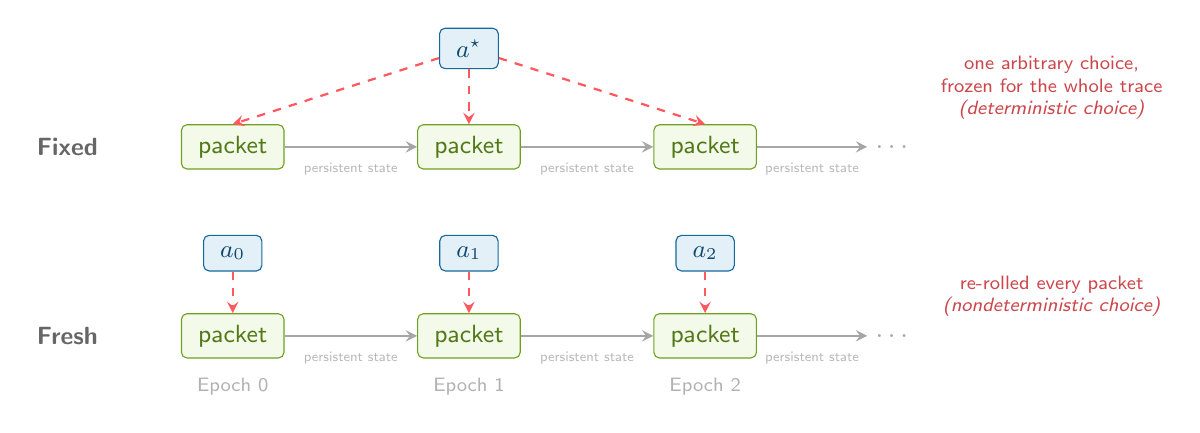
\begin{tikzpicture}[
      box/.style={rounded corners=2pt, draw, font=\small\sffamily, inner xsep=6pt, inner ysep=4pt},
      pkt/.style={box, fill=palOlivine!10, draw=palOlivine!80!black, text=palOlivine!60!black},
      act/.style={box, fill=palCerulean!12, draw=palCerulean!80!black, text=palCerulean!55!black, font=\small\sffamily},
      arw/.style={->, >=stealth, thick, draw=gray!70},
      feed/.style={->, >=stealth, dashed, palCoral, thick},
      rowlab/.style={font=\bfseries\sffamily\small, text=gray!80!black}
    ]

    % ---- Fixed band (top) -------------------------------------------------
    \node[rowlab] at (-2.1, 2.0) {Fixed};
    \foreach \i/\x in {0/0, 1/3, 2/6} {
      \node[pkt] (fp\i) at (\x, 2.0) {packet};
    }
    \node[font=\bfseries\sffamily, text=gray!70] at (8.4, 2.0) {$\dots$};
    \draw[arw] (fp0.east) -- node[midway, below=2pt, font=\tiny\sffamily, text=gray!55] {persistent state} (fp1.west);
    \draw[arw] (fp1.east) -- node[midway, below=2pt, font=\tiny\sffamily, text=gray!55] {persistent state} (fp2.west);
    \draw[arw] (fp2.east) -- node[midway, below=2pt, font=\tiny\sffamily, text=gray!55] {persistent state} ++(1.4,0);

    \node[act] (astar) at (3, 3.25) {$a^{\star}$};
    \foreach \i in {0,1,2} { \draw[feed] (astar) -- (fp\i.north); }
    \node[font=\scriptsize\sffamily, text=palCoral!80!black, align=center] at (10.4, 2.75)
      {one arbitrary choice,\\ frozen for the whole trace\\ \emph{(deterministic choice)}};

    % ---- Fresh band (bottom) ----------------------------------------------
    \node[rowlab] at (-2.1, -0.4) {Fresh};
    \foreach \i/\x in {0/0, 1/3, 2/6} {
      \node[pkt] (sp\i) at (\x, -0.4) {packet};
      \node[act] (sa\i) at (\x, 0.65) {$a_{\i}$};
      \draw[feed] (sa\i) -- (sp\i.north);
    }
    \node[font=\bfseries\sffamily, text=gray!70] at (8.4, -0.4) {$\dots$};
    \draw[arw] (sp0.east) -- node[midway, below=2pt, font=\tiny\sffamily, text=gray!55] {persistent state} (sp1.west);
    \draw[arw] (sp1.east) -- node[midway, below=2pt, font=\tiny\sffamily, text=gray!55] {persistent state} (sp2.west);
    \draw[arw] (sp2.east) -- node[midway, below=2pt, font=\tiny\sffamily, text=gray!55] {persistent state} ++(1.4,0);
    \node[font=\scriptsize\sffamily, text=palCoral!80!black, align=center] at (10.4, 0.1)
      {re-rolled every packet\\ \emph{(nondeterministic choice)}};

    % epoch ticks
    \foreach \i/\x in {0/0, 1/3, 2/6} {
      \node[font=\scriptsize\sffamily, text=gray!60] at (\x, -1.05) {Epoch \i};
    }

  \end{tikzpicture}

  \vspace{0.5em}
  \begin{itemize}\small\setlength\itemsep{0.3em}
    \item For concrete execution we turn each table's action choice into the trivial table entry that selects exactly that action.
  \end{itemize}
\end{frame}


% \begin{frame}{Reactive Controller Language}
%   At the start of each epoch the controller runs a \texttt{CPProgram}, an ordinary Core block instantiated at the control-plane extension \texttt{CPExt}. It reuses Core's control flow (\texttt{if}, \texttt{for}, \texttt{block}, \texttt{assign}), the whole expression language, and register, counter and meter reads \emph{verbatim}. Only the table operations are new.

%   \vspace{0.5em}
%   \begin{columns}[T,onlytextwidth]
%     \begin{column}{0.56\textwidth}
%       \begin{block}{The \texttt{CPExt} constructs}
%         \small
%         \setlength\tabcolsep{4pt}
%         \renewcommand{\arraystretch}{1.25}
%         \begin{tabular}{@{}ll@{}}
%           \texttt{\textcolor{palCerulean!70!black}{add}}\,($t$, $e$)
%             & install entry $e$ into table $t$ \\
%           \texttt{remove}\,($t$, $k$, $p$)
%             & delete entry matching key $k$ \\
%           \texttt{modify}\,($t$, $k$, $p$, $a$)
%             & re-point key $k$ to action $a$ \\
%           \texttt{setDefault}\,($t$, $a$)
%             & set $t$'s default action \\
%           \texttt{\textcolor{palCoral!75!black}{havoc}}\,($t$)
%             & re-choose $t$ \emph{arbitrarily} \\
%           \texttt{\textcolor{palCoral!75!black}{havocAll}}
%             & re-choose \emph{every} table \\
%           \texttt{skip}
%             & no-op \\
%         \end{tabular}
%       \end{block}
%     \end{column}

%     \begin{column}{0.42\textwidth}
%       \footnotesize
%       \textbf{\textcolor{palCoral!75!black}{havoc}} is the symbolic abstraction. With no controller supplied, \texttt{havocAll} over-approximates \emph{all} reachable table configurations in one symbolic state.
%       \vspace{0.6em}

%       \textbf{\textcolor{palCerulean!70!black}{add}} / \texttt{remove} / \texttt{modify} are the concrete entries-model edits. Their keys, entries and actions reuse the Core entry vocabulary, so payloads are plain Core expressions.
%     \end{column}
%   \end{columns}

%   \vspace{0.4em}
%   \begin{block}{Reacting to carried state}
%     \footnotesize
%     Reading the carried persistent state lets the controller react. For example, install a drop rule once a counter crosses a threshold.
%     \[
%       \texttt{when}\;(\,\texttt{reg}[\,\mathtt{0}\,] > \mathtt{100}\,)\;\;
%       [\;\texttt{add}\;\mathit{acl}\;\mathit{dropEntry}\;]
%     \]
%   \end{block}
% \end{frame}

\begin{frame}{The Specification Language}
  We layer an \LTL{} specification language over \emph{intra-packet atoms}, the observations of a single packet execution.
  \par
  \vspace{-0.2em}
  \begin{columns}[t]
    \begin{column}{0.5\textwidth}
      \[
      \begin{array}{rcl}
        \multicolumn{3}{l}{\textbf{Intra-packet atom}}\\[3pt]
        \specAtom &::=&  \mathbf{if}\ \specAtom\ \mathbf{then}\ \specAtom\ [\mathbf{else}\ \specAtom] \\[2pt]
                  &\mid& \lnot \specAtom \mid \specAtom \oplus \specAtom \mid \specExpr \\[2pt]
                  &\mid& \specExpr @ \specLoc \mid \specHit @ \specBlock \mid \specDrop \\[2pt]
                  &\mid& \mathit{port\_in} \mid \mathit{port\_out}
      \end{array}
      \]
    \end{column}
    \begin{column}{0.5\textwidth}
      \[
      \begin{array}{rcl}
        \multicolumn{3}{l}{\textbf{LTL path formula}}\\[3pt]
        \ltlFormula &::=& \specAtom \mid \lnot \ltlFormula \mid \ltlFormula_1 \land \ltlFormula_2 \\[2pt]
                    &\mid& \Next \ltlFormula \mid \ltlFormula_1 \Until \ltlFormula_2 \\[8pt]
        \multicolumn{3}{l}{\textbf{Specification}}\\[3pt]
        \Phi &::=& \forall x{:}\tau.\ \Phi \mid \ltlFormula
      \end{array}
      \]
    \end{column}
  \end{columns}

  \vspace{0.3em}
  \raggedright\footnotesize
  \begin{itemize}\setlength\itemsep{2pt}
    \item \(\specExpr\) is a P4 expression. An \(@\specLoc\) suffix captures its value at a
          program location \(\specLoc = \specBlock.\specBegin \mid \specBlock.\specEnd\),
          where \(\specBlock\) is a control block, table or action; without \(@\specLoc\) it
          must be a constant.
    \item \(\specDrop\) holds when a packet produces zero outputs, \(\specHit @ \specBlock\)
          asserts control flow reaches \(\specBlock\), and \(\mathit{port\_in}\,/\,\mathit{port\_out}\)
          are the ingress\,/\,egress ports of the current packet.
    \item The leading binder \(\forall x{:}\tau.\) introduces a rigid symbolic value fixed
          across all steps.
  \end{itemize}
\end{frame}

\begin{frame}{Temporal Logic (\LTL{}) by Example}
  In our model ``time'' advances one step every time a new packet enters the
  switch, so a formula talks about the infinite sequence of packets. The grammar
  keeps only \(\Next\) and \(\Until\) primitive. The familiar operators are
  derived shorthand on top of those two.

  \vspace{0.5em}
  \begin{itemize}\setlength\itemsep{6pt}
    \item \(\Next\,\varphi\) (next), the property holds for the very next packet.
    \item \(\Until\) (until), one property keeps holding right up to the packet
          where a second one takes over.
    \item \(\Eventually\,\varphi\) (eventually), the property holds for some
          packet now or later.
    \item \(\Globally\,\varphi\) (globally), the property holds for every packet
          from now on.
    \item \(\WeakUntil\) (weak until), like until, but the second property is
          allowed to never arrive.
  \end{itemize}

  \vspace{0.4em}
  \raggedright\footnotesize
  \textbf{Properties a P4 author might write}
  \begin{itemize}\setlength\itemsep{5pt}
    \item \(\Globally\,(\lnot\,\specDrop \rightarrow \specHit@\mathit{acl})\),
          no packet is forwarded without the ACL table being reached.
    \item \(\Globally\,((\texttt{hdr.ipv4.ttl} == 0)@\texttt{ingress}.\specEnd
          \rightarrow \specDrop)\), a packet whose TTL has reached zero is
          dropped, never forwarded.
  \end{itemize}
\end{frame}

\begin{frame}{Verification Approach}
  P4Check runs one engine, combining \textbf{bounded model checking} and
  \textbf{k-induction}, that both proves and refutes full \LTL{} over an infinite
  packet trace. An iterative-deepening driver reduces every property shape to the
  reachability of a \emph{bad} state.

  \vspace{0.9em}
  \begin{itemize}\setlength\itemsep{0.9em}
    \item \textbf{Safety} \(\Globally\, p\). Already a reachability question,
          checked directly.
    \item \textbf{Liveness} \(\Eventually\, p,\ \Globally\Eventually\, p\). A
          liveness-to-safety monitor turns an accepting \emph{lasso} into a
          reachable bad state.
    \item \textbf{Full \LTL{}}. The negation compiles to a B\"uchi automaton run
          in product with the system, and its accepting lasso again becomes a
          reachable bad state.
  \end{itemize}

  \vspace{0.9em}
  At each depth \(k\), \(\textsc{Base}_k\)
  \textcolor{palCoral!75!black}{\textbf{SAT}} returns a bounded looping
  counterexample (\textbf{Refuted}) and \(\textsc{Step}_k\)
  \textcolor{palOlivine!60!black}{\textbf{UNSAT}} under a simple-path constraint
  is a proof (\textbf{Proved}).
\end{frame}

\begin{frame}{K-Induction in One Slide}
  Prove a safety invariant \(\Globally\, p\), where \(p\) is a per-packet
  predicate and one step runs one packet, \(R_{i+1} = \mathit{step}(R_i)\). At
  each depth \(k\) the engine builds two queries.

  \vspace{0.7em}
  \begin{columns}[T,onlytextwidth]
    \begin{column}{0.49\textwidth}
      \begin{block}{Base case at depth \(k\)}
        \small
        Is there a \emph{real} counterexample within \(k\) steps of the true
        initial state?
        \[
          \mathrm{Base}(k)\;=\;\bigvee_{i=0}^{k-1} \lnot p(R_i)
        \]
        \(R_0\) is the device init seed, which is \textbf{target-specific}.
        \par\vspace{0.4em}
        \textcolor{palCoral!75!black}{\textbf{SAT}} \(\Rightarrow\)
        \textbf{Refuted}, a genuine counterexample.
      \end{block}
    \end{column}

    \begin{column}{0.49\textwidth}
      \begin{block}{Step case at depth \(k\)}
        \small
        Can \(p\) break after \(k\) good steps from an \emph{arbitrary} state?
        \[
          \mathrm{Step}(k)\;=\;\bigwedge_{i=0}^{k-1} p(R_i)\;\wedge\;\lnot p(R_k)
        \]
        \(R_0\) is a fresh \textbf{well-formed} state, structurally valid but
        \emph{not necessarily reachable}, with the states kept pairwise distinct
        (a \emph{simple path}).
        \par\vspace{0.4em}
        \textcolor{palOlivine!60!black}{\textbf{UNSAT}} \(\Rightarrow\)
        \textbf{Proved}.
      \end{block}
    \end{column}
  \end{columns}

  \vspace{0.6em}
  \footnotesize
  Deepen \(k = 1, 2, \dots, \text{maxK} = 8\). \(\mathrm{Base}(k)\) SAT is
  \textbf{Refuted} and \(\mathrm{Step}(k)\) UNSAT is \textbf{Proved}. A failing
  \(\mathrm{Step}\) can be \emph{spurious}, because the arbitrary \(R_0\) need
  not be reachable, so it only forces a deeper \(k+1\). If none closes by
  \(\text{maxK}\), the verdict is \textbf{Unknown}.
\end{frame}



% \input{pipeline.tex}

% Concrete payoff of the previous slide. Same program, same one-packet
% transition. The ONLY thing that changes between the two targets is R0 in the
% BASE: bmv2 pins it to 0 (ZeroInit, Level-2 device fact), the abstract v1model
% leaves it arbitrary (UndefinedInit, Level 1). Grounded in src2 Verify.Engine
% (deepen / invariantQueries) and Runtime.Target (RegisterInitPolicy), maxK = 8.
\begin{frame}{K-Induction by Example}
  \centering
  \small
  \begin{minipage}{0.96\textwidth}\centering
    \ttfamily\footnotesize
    register<bit<8>{}>(1) r;\qquad apply \{ r.write(0, r.read(0) + 2); \}
  \end{minipage}
  \par\vspace{0.3em}
  Prove \(\Globally\,(r \neq 7)\) for register \(r\), whose value after \(i\)
  packets is \(R_i\). Each packet runs \(R_{i+1} = R_i + 2 \pmod{256}\).
  \par\vspace{0.1em}
  {\footnotesize The transition is identical on both targets. The \emph{only}
   difference is \(R_0\), the \textsc{Base} init seed.}

  \vspace{0.6em}
  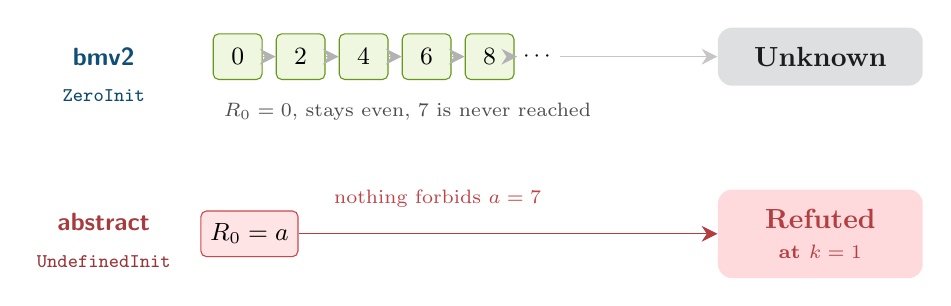
\begin{tikzpicture}[
      font=\footnotesize,
      cell/.style={rounded corners=2pt, draw, minimum width=0.62cm, minimum height=0.58cm, font=\small},
      good/.style={cell, fill=palOlivine!14, draw=palOlivine!75!black},
      seed/.style={cell, minimum width=1.05cm, fill=palCoral!16, draw=palCoral!80!black},
      tedge/.style={-{Stealth[length=2mm,width=2mm]}, draw=gray!60},
      lane/.style={font=\bfseries\sffamily\small, align=left},
      verdict/.style={rounded corners=5pt, font=\bfseries, inner sep=7pt, minimum width=2.6cm, align=center}
    ]
    % ---- Lane A: bmv2 / ZeroInit -> Unknown -------------------------------
    \node[lane, text=palCerulean!60!black] at (-0.4,0.55) {bmv2};
    \node[font=\scriptsize\ttfamily, text=palCerulean!55!black] at (-0.4,0.05) {ZeroInit};
    \foreach \v/\x [count=\i from 0] in {0/1.3, 2/2.1, 4/2.9, 6/3.7, 8/4.5}
      \node[good] (a\i) at (\x,0.55) {\v};
    \foreach \i/\j in {0/1,1/2,2/3,3/4} \draw[tedge] (a\i) -- (a\j);
    \node at (5.1,0.55) {\(\cdots\)};
    \draw[tedge] (a4) -- (4.85,0.55);
    \node[font=\scriptsize, text=gray!60!black, anchor=west] at (1.0,-0.15)
      {\(R_0 = 0\), stays even, \(7\) is never reached};
    \node[verdict, fill=palGray!22, text=palGray!25!black] (vA) at (8.7,0.55) {Unknown};
    \draw[tedge, gray!45] (5.4,0.55) -- (vA.west);

    % ---- Lane B: abstract / UndefinedInit -> Refuted ----------------------
    \node[lane, text=palCoral!65!black] at (-0.4,-1.55) {abstract};
    \node[font=\scriptsize\ttfamily, text=palCoral!60!black] at (-0.4,-2.05) {UndefinedInit};
    \node[seed] (b0) at (1.45,-1.7) {\(R_0 = a\)};
    \node[font=\scriptsize, text=palCoral!75!black, anchor=west] at (2.4,-1.25)
      {nothing forbids \(a = 7\)};
    \node[verdict, fill=palCoral!22, text=palCoral!70!black] (vB) at (8.7,-1.7)
      {Refuted\\[-1pt]\scriptsize at \(k = 1\)};
    \draw[tedge, draw=palCoral!70!black] (b0) -- (vB.west);
  \end{tikzpicture}

  \vspace{0.5em}
  \begin{columns}[T,onlytextwidth]
    \begin{column}{0.5\textwidth}
      \footnotesize
      \textbf{\textcolor{palCerulean!60!black}{bmv2}}.\;
      \(\mathrm{Base}(k)\) is always \textcolor{palOlivine!60!black}{UNSAT}, no
      real counterexample. But the \(\mathrm{Step}\) re-seeds \(R_0\) freely and
      escapes into odd states (\(5{\to}7,\ 3{\to}5{\to}7,\dots\)) it cannot rule
      out by \(k = 8\).
    \end{column}
    \begin{column}{0.5\textwidth}
      \footnotesize
      \textbf{\textcolor{palCoral!65!black}{abstract}}.\;
      \(\mathrm{Base}(1) = \lnot p(R_0) = (a = 7)\) is
      \textcolor{palCoral!75!black}{SAT}. The register may power on at \(7\), so
      the property genuinely fails before any packet matters.
    \end{column}
  \end{columns}
\end{frame}

% Proof-by-Step counterpart of the refutation example. SAME program and target
% (bmv2 / ZeroInit) as the previous slide, only the property changes: G(r even)
% is 1-inductive so STEP proves it at k=1, whereas G(r != 7) is not inductive
% and STEP never closes (-> Unknown). Shows k-induction actually PROVING (BASE
% alone can never prove), grounded in src2 Verify.Engine (deepen / Step UNSAT =>
% Proved).
\begin{frame}{K-Induction by Example (Proof by Step)}
  \centering
  \small
  \begin{minipage}{0.96\textwidth}\centering
    \ttfamily\footnotesize
    register<bit<8>{}>(1) r;\qquad apply \{ r.write(0, r.read(0) + 2); \}
  \end{minipage}
  \par\vspace{0.3em}
  Same program on \textbf{\textcolor{palCerulean!60!black}{bmv2}}, now prove
  \(\Globally\,(r\ \text{even})\) with predicate \(p(R_i) = (R_i \bmod 2 = 0)\).

  \vspace{0.7em}
  \begin{columns}[T,onlytextwidth]
    \begin{column}{0.49\textwidth}
      \begin{block}{Base alone cannot prove}
        \small
        \[ \mathrm{Base}(k) = \bigvee_{i=0}^{k-1}\lnot p(R_i) \]
        is \textcolor{palOlivine!60!black}{\textbf{UNSAT}}, since
        \(0, 2, 4, \dots\) are all even. But that only says \emph{no violation
        within \(k\) steps}, never that none ever happens.
      \end{block}
    \end{column}

    \begin{column}{0.49\textwidth}
      \begin{block}{Step proves at \(k = 1\)}
        \small
        Assume \(p(R_0)\), so \(R_0\) is even. Then \(R_1 = R_0 + 2\) is even, so
        \[ \mathrm{Step}(1) = p(R_0) \wedge \lnot p(R_1) \]
        is \textcolor{palOlivine!60!black}{\textbf{UNSAT}} \(\Rightarrow\)
        \textbf{Proved}.
      \end{block}
    \end{column}
  \end{columns}

  \vspace{0.5em}
  \begin{block}{Same program and target, two properties}
    \footnotesize
    \(\Globally\,(r\ \text{even})\) is \textbf{inductive}, evenness is preserved
    from \emph{any} start, so \(\textsc{Step}\) proves it at \(k = 1\).
    \(\Globally\,(r \neq 7)\) is \textbf{not inductive}, an arbitrary odd
    \(R_0\) reaches \(7\) (\(5{\to}7,\ 3{\to}5{\to}7,\dots\)), so \(\textsc{Step}\)
    never closes and the verdict is \textbf{Unknown}. Inductiveness, decided by
    \(\textsc{Step}\), is what separates the two.
  \end{block}
\end{frame}

% \input{pipeline.tex}

\section{Debugging}

% Progress-marker: highlight the Trace + Debugger region, the concrete-mode
% output that the debugging part of the talk builds on.
\begin{frame}{Architecture: Debugging}
\centering
\resizebox{\linewidth}{!}{%
  \begingroup
  \def\PFourArchOverlay{%
    \draw[palCoral, line width=1.6pt, rounded corners=6pt]
      ([xshift=-0.22cm, yshift=0.18cm]trace.west |- debugger.north)
      rectangle
      ([xshift=0.24cm, yshift=-0.20cm]debugger.south east);
  }%
  \begingroup%
% Canonical geometry for this figure. Keep these definitions local so callers
% cannot accidentally change the rendered aspect ratio before inputting it.
\def\PFourArchBoxXSep{0.08cm}%
\def\PFourInstrumentBelowFrontend{0.65cm}%
\def\PFourToolStageWidth{1.58cm}%
\def\PFourVerifyAfterInstrument{0.5cm}%
\def\PFourLocalizeBelowCounterexample{0.75cm}%
\def\PFourVerifyResultXSep{0.40cm}%
\def\PFourResultArtifactXSep{0.75cm}%
\def\PFourOutputArtifactXSep{0.25cm}%
\def\PFourArchBoxYSep{0.08cm}%
\def\PFourSymbolicBandPad{0.08cm}%
% Fonts: use the deck's default font (no biolinum), keep zi4 for monospace.
\def\PFourArchText{\fontsize{6}{7}\selectfont}%
\def\PFourArchTiny{\fontsize{5}{6}\selectfont}%
\def\PFourArchMonoTiny{\fontencoding{T1}\fontfamily{zi4}\fontsize{5}{6}\selectfont}%
\def\PFourArchLarge{\fontsize{10}{12}\selectfont}%
\begin{tikzpicture}[
    font=\PFourArchText,
    >=Latex,
    box/.style={
        rectangle,
        draw=black!70,
        fill=white,
        align=center,
        minimum height=0.72cm,
        inner xsep=4pt,
        inner ysep=3pt
    },
    inputbox/.style={
        ellipse,
        draw=black!70,
        fill=palOlivine!25,
        align=center,
        minimum width=1.45cm,
        minimum height=0.58cm,
        inner xsep=4pt,
        inner ysep=2pt
    },
    stage/.style={
        box,
        fill=palGray!12,
        minimum width=1.20cm
    },
    toolstage/.style={
        stage,
        minimum width=\PFourToolStageWidth,
        text width=1.28cm,
        align=center
    },
    artifact/.style={
        ellipse,
        draw=black!70,
        fill=palCoral!22,
        align=center,
        minimum width=1.35cm,
        minimum height=0.58cm,
        inner xsep=4pt,
        inner ysep=2pt
    },
    compactartifact/.style={
        artifact,
        font=\PFourArchTiny,
        minimum width=1.30cm,
        minimum height=0.50cm,
        inner xsep=2.5pt,
        inner ysep=1.5pt
    },
    widebox/.style={
        box,
        fill=palGray!7,
        minimum width=2.86cm
    },
    semblock/.style={
        box,
        fill=white,
        font=\PFourArchTiny,
        minimum width=0.93cm,
        minimum height=0.48cm,
        inner xsep=3pt,
        inner ysep=2pt
    },
    note/.style={
        font=\PFourArchText\bfseries,
        align=center
    },
    arrow/.style={
        -{Latex[length=2mm]},
        line width=0.45pt,
        shorten >=1pt,
        shorten <=1pt
    },
    dataarrow/.style={
        arrow,
        dashed,
        draw=black!65
    },
    semarrow/.style={
        -{Latex[length=1.4mm]},
        line width=0.35pt,
        shorten >=1pt,
        shorten <=1pt
    }
]

% Inputs.
\node[inputbox] (source) at (0,2.85) {P4 Source\\Code};

% Frontend.
\node[box, minimum width=1.55cm, minimum height=2.10cm, fill=palGray!9, anchor=north]
    (frontend) at (2.0,3.575) {};
\node[note, anchor=north] at (frontend.north) {Frontend};
\node[stage] (parser) at (2.0,2.86) {Parser};
\node[stage] (ast) at (2.0,1.96) {AST};
\node[toolstage, anchor=north] (instrument)
    at ([yshift=-\PFourInstrumentBelowFrontend]frontend.south) {Instrument};
\node[inputbox] (property) at (source.center |- instrument.center) {Property};

% Haskell implementation.
\node[widebox, minimum height=1.48cm]
    (interpreter) at (4.65,2.77) {};
\node[note, anchor=north] (interp-title) at (interpreter.north) {Interpreter};
\path[fill=palCitron, opacity=0.55]
    let \p1 = (interpreter.south west) in
    (\x1,\y1) rectangle (9.48cm,3.52cm);
\path let \p1 = (interpreter.south west) in
    node[note, anchor=south, yshift=0.05cm]
    at ($(\x1,3.52cm)!0.5!(9.48cm,3.52cm)$) {Concrete mode (Debugging)};
\node[font=\PFourArchTiny, align=center] at ([yshift=0.08cm]interpreter.center)
    {Unified: Concrete \& Symbolic};
\node[semblock] (staticsem) at ([xshift=-0.58cm,yshift=-0.42cm]interpreter.center)
    {Static\\Semantics};
\node[semblock] (dynamicsem) at ([xshift=0.58cm,yshift=-0.42cm]interpreter.center)
    {Dynamic\\Semantics};
\draw[semarrow] (staticsem.east) -- (dynamicsem.west);

% Concrete/debugging outputs.
\node[box, minimum width=1.22cm, minimum height=0.96cm, inner sep=0pt]
    (debugger) at (8.65,2.77) {};
\node[compactartifact, minimum width=0.82cm, minimum height=0.42cm,
    inner xsep=2pt, inner ysep=1pt]
    (trace) at ($(interpreter.east)!0.5!(debugger.west)$) {Trace};
\path[fill=palGray!22, draw=black!65, line width=0.22pt]
    ([xshift=-0.61cm,yshift=0.34cm]debugger.center)
    rectangle ++(1.22cm,0.14cm);
\fill[palCoral!80!black]
    ([xshift=-0.53cm,yshift=0.41cm]debugger.center) circle (0.018cm);
\node[font=\PFourArchMonoTiny, anchor=east]
    at ([xshift=0.54cm,yshift=0.41cm]debugger.center) {\textless\ \textgreater};
\draw[line width=0.18pt, draw=black!40]
    ([xshift=-0.34cm,yshift=0.30cm]debugger.center) -- ++(0,-0.55cm);
\fill[palCitron]
    ([xshift=-0.30cm,yshift=0.12cm]debugger.center)
    rectangle ++(0.80cm,0.12cm);
\node[font=\PFourArchMonoTiny, text=black!50, anchor=west]
    at ([xshift=-0.47cm,yshift=0.18cm]debugger.center) {1};
\node[font=\PFourArchMonoTiny, text=black!50, anchor=west]
    at ([xshift=-0.47cm,yshift=0.05cm]debugger.center) {2};
\node[font=\PFourArchMonoTiny, text=black!50, anchor=west]
    at ([xshift=-0.47cm,yshift=-0.08cm]debugger.center) {3};
\node[font=\PFourArchMonoTiny, text=black!50, anchor=west]
    at ([xshift=-0.47cm,yshift=-0.21cm]debugger.center) {4};
\node[font=\PFourArchMonoTiny, anchor=west]
    at ([xshift=-0.24cm,yshift=0.18cm]debugger.center) {if(hit)};
\node[font=\PFourArchMonoTiny, anchor=west]
    at ([xshift=-0.14cm,yshift=0.05cm]debugger.center) {apply};
\node[font=\PFourArchMonoTiny, anchor=west]
    at ([xshift=-0.24cm,yshift=-0.08cm]debugger.center) {else};
\node[font=\PFourArchMonoTiny, anchor=west]
    at ([xshift=-0.14cm,yshift=-0.21cm]debugger.center) {drop};
\fill[palCoral!80!black]
    ([xshift=-0.52cm,yshift=0.18cm]debugger.center) circle (0.026cm);
\draw[line width=0.22pt, draw=black!65]
    ([xshift=-0.61cm,yshift=-0.28cm]debugger.center) -- ++(1.22cm,0);
\node[font=\PFourArchMonoTiny, anchor=west]
    at ([xshift=-0.48cm,yshift=-0.38cm]debugger.center) {pkt};
\node[font=\PFourArchMonoTiny, anchor=west]
    at ([xshift=0.10cm,yshift=-0.38cm]debugger.center) {meta};
% Concrete mode label moved to yellow band path

% Symbolic/verification outputs.
\node[toolstage, anchor=west]
    (verify) at ([xshift=\PFourVerifyAfterInstrument,yshift=0.45cm]instrument.east) {Verify};
\node[font=\PFourArchLarge\bfseries, text=palOlivine!80!black, inner sep=1pt]
    (verifyok) at ([xshift=\PFourVerifyResultXSep,yshift=-0.28cm]verify.east) {\ding{51}};
\node[font=\PFourArchLarge\bfseries, text=palCitron!65!black, inner sep=1pt]
    (verifyunknown) at ([xshift=\PFourVerifyResultXSep]verify.east) {?};
\node[font=\PFourArchLarge\bfseries, text=palCoral!85!black, inner sep=1pt]
    (verifyfail) at ([xshift=\PFourVerifyResultXSep,yshift=0.28cm]verify.east) {\ding{55}};
\node[compactartifact, anchor=west]
    (counterexample) at ([xshift=\PFourResultArtifactXSep]verifyfail.east)
    {Counter-\\example};
\node[compactartifact, anchor=west]
    (propbreakpoint)
    at ([xshift=\PFourOutputArtifactXSep,yshift=-\PFourLocalizeBelowCounterexample]counterexample.east)
    {Breakpoint};
% Symbolic mode label moved to red band path

% Main flow.
\draw[arrow] (source.east) -- (parser.west);
\draw[arrow] (parser.south) -- (ast.north);
\draw[arrow] (ast.east) -- ++(0.30,0) |- (interpreter.west);
\draw[arrow] (interpreter.east) -- (trace.west);
\draw[arrow] (trace.east) -- (debugger.west);

% Instrumentation and verification flow.
\draw[dataarrow] (property.east) -- (instrument.west);
\draw[dataarrow] (frontend.south) -- (instrument.north);
\draw[dataarrow] (instrument.east) -- ++(0.26,0) -- ++(0,1.12) -| ([xshift=-1.0cm]interpreter.south);
\draw[dataarrow] ([xshift=0.35cm]interpreter.south) -- ++(0,-0.35) -| (verify.north);
\draw[dataarrow] (verify.east |- verifyfail.center) -- (verifyfail.west);
\draw[dataarrow] (verify.east |- verifyunknown.center) -- (verifyunknown.west);
\draw[dataarrow] (verify.east |- verifyok.center) -- (verifyok.west);
\draw[dataarrow] (verifyfail.east) -- (counterexample.west);
\draw[dataarrow] (property.south) -- ++(0,-0.5) -| ([xshift=-0.28cm]propbreakpoint.south);
\draw[dataarrow] (counterexample.north) -- ++(0,0.30)
    -| ([xshift=1.05cm]interpreter.south);
\draw[dataarrow] (propbreakpoint.north) --
    (propbreakpoint.north |- debugger.south);

\begin{scope}[on background layer]
    \path[fill=palCerulean!90, opacity=0.22]
        let
            \p1 = (interpreter.west),
            \p2 = ([yshift=-\PFourSymbolicBandPad]propbreakpoint.south),
            \p3 = ([yshift=\PFourSymbolicBandPad]counterexample.north)
        in
            (\x1,\y2) rectangle (9.48cm,\y3);
\end{scope}
% Place label below the red band using relative offset from its bottom edge
\path let
        \p1 = (interpreter.west),
        \p2 = ([yshift=-\PFourSymbolicBandPad]propbreakpoint.south)
    in
    node[note, anchor=north, yshift=-0.05cm]
    at ($(\x1,\y2)!0.5!(9.48cm,\y2)$) {Symbolic model (Verification)};

% Overlay hook: if the caller defined \PFourArchOverlay, execute it now.
% This lets progress-marker slides highlight parts of the diagram without
% duplicating the figure source.
\ifdefined\PFourArchOverlay\PFourArchOverlay\fi

\pgfresetboundingbox
\path[use as bounding box] (-0.90,-0.45) rectangle (9.70,3.95);

\end{tikzpicture}%
\endgroup%
%
  \endgroup
}
\end{frame}

\begin{frame}{Debugging with Breakpoints}
  The concrete execution is instrumented to capture a step at every statement,
  giving a finite trace of \emph{events}. A breakpoint is a small query over
  that trace, a two-layer algebra that names \emph{where} to stop.

  \vspace{0.1em}
  \begin{columns}[t,onlytextwidth]
    \begin{column}{0.42\textwidth}
      \footnotesize\textbf{Event predicate}\ (one step)
      \vspace{-0.4em}
      \[
      \begin{array}{rcl}
        \varphi &::=& (\specExpr) \ \mid\ @\specLoc \\[2pt]
                &\mid& \varphi \land \varphi \ \mid\ \varphi \lor \varphi \\[2pt]
                &\mid& \lnot\varphi \ \mid\ \mathsf{true}
      \end{array}
      \]
      \vspace{-0.3em}
      \footnotesize\textbf{Breakpoint}\ (where to stop)
      \vspace{-0.4em}
      \[
      \begin{array}{rcl}
        b &::=& \mathbf{when}\ \varphi \\[3pt]
          &\mid& \varphi \mathrel{\mathbf{until}} \psi \\[3pt]
          &\mid& b \mathrel{\mathbf{after}} \varphi \\[3pt]
          &\mid& b \mathrel{\mathbf{before}} \varphi
      \end{array}
      \]
    \end{column}
    \begin{column}{0.56\textwidth}
      \scriptsize
      \begin{itemize}\setlength\itemsep{3.5pt}
        \item $(\specExpr)$ a \textbf{data test}, a P4 boolean expression read off
              the step's state; $@\specLoc$ a \textbf{structural test}, control
              reaches $\specLoc = \specBlock.\specBegin \mid \specBlock.\specEnd$
              (a block, table or action; or a source line).
        \item $\mathbf{when}\ \varphi$ stop the \textbf{first time} $\varphi$
              becomes true, a \emph{watchpoint}.
        \item $\varphi \mathrel{\mathbf{until}} \psi$ $\varphi$ holds up to
              $\psi$; stop on $\varphi$'s \textbf{rising edge}. (The classic
              $\specExpr@\specLoc$ is just $(\specExpr) \mathrel{\mathbf{until}} @\specLoc$.)
        \item $b \mathrel{\mathbf{after}} \varphi$ a \textbf{gate}: ignore steps
              until $\varphi$ has happened, then run $b$.
        \item $b \mathrel{\mathbf{before}} \varphi$ a \textbf{deadline}: $b$ must
              fire at or before $\varphi$, otherwise it misses.
      \end{itemize}
    \end{column}
  \end{columns}

  \vspace{0.1em}
  \footnotesize
  \textbf{Same step vs.\ across steps.}\ $\land$ asks \emph{one} event to pass
  both tests at once; $\mathbf{after}$ / $\mathbf{before}$ are \emph{temporal},
  relating \emph{different} events along the trace.

  \vspace{0.2em}
  {\scriptsize\ttfamily std.egress\_spec == 9w511}\ {\scriptsize\textcolor{palGray}{stops where the packet is first marked for drop.}}
\end{frame}

{
\setbeamertemplate{headline}{}
\setbeamertemplate{footline}{}
\begin{frame}[plain]
  \centering
  \vfill
  {\Huge\textbf{Demo}}
  \vfill
\end{frame}
}



\section{Evaluation}

\begin{frame}{Validation: Do we model P4?}
  \vspace{0.4em}
  To validate the correctness of the interpreter, we test both the concrete and symbolic paths.

  \vspace{0.8em}
  \begin{columns}[T,onlytextwidth]
    \begin{column}{0.48\textwidth}
      \begin{block}{Concrete Interpreter}
        \small
        \begin{itemize}\setlength\itemsep{6pt}
          \item p4c testsuite: passes 80\%
          \item P4TestGen~\cite{10.1145/3603269.3604834} on real-world programs: 40\%
          % \item Generate expected input-output pairs for each possible control flow path.
          % \item Verify that P4Check produces matching results.
        \end{itemize}
      \end{block}
    \end{column}

    \begin{column}{0.48\textwidth}
      \begin{block}{Symbolic Interpreter}
        \small
        \begin{itemize}\setlength\itemsep{6pt}
          \item Generate input-output pairs for real programs from the symbolic execution
          \item Compare with HOL4P4 and P4SpecTec
        \end{itemize}
      \end{block}
    \end{column}
  \end{columns}

  \vspace{0.6em}
  \centering
  \textcolor{palOlivine!60!black}{\checkmark}\ \textbf{Result:} Still some more modeling to do.
\end{frame}

\newcommand{\rgood}[1]{\textcolor{palOlivine!65!black}{\ding{51}}\,{\tiny#1}}
\newcommand{\rbad}[1]{\textcolor{palCoral}{\ding{55}}\,{\tiny#1}}
\newcommand{\rto}[1]{\textcolor{palCoral}{timeout}\,{\tiny#1}}
\newcommand{\rerr}[1]{\textcolor{palCoral}{error}\,{\tiny#1}}
\newcommand{\runk}[1]{\textcolor{palGray}{unknown}\,{\tiny#1}}
\newcommand{\rna}{\textcolor{palGray}{n/a}}
\begin{frame}{Verification Performance Numbers}
  \centering
  \scriptsize
  \setlength{\tabcolsep}{4.5pt}
  \renewcommand{\arraystretch}{1.18}



  \begin{tabular}{@{}l l l l l@{}}
    \toprule
    \textbf{Phase} & \textbf{Property} & \textbf{P4TV} & \textbf{p4check2} & \textbf{assert-p4} \\
    \midrule
    trivial  & \texttt{never-drops}                       & \rgood{(4495 ms)}    & \rgood{(665 ms)}    & \rgood{(215 ms)} \\
    \addlinespace[2pt]
    intra    & \texttt{handle-1a-produces-1b}               & \rgood{(16409 ms)}   & \rgood{(1675 ms)}   & \rna \\
    intra    & \texttt{deliver-requires-majority}           & \rerr{(4010 ms)}     & \rgood{(1045 ms)}   & \rna \\
    intra    & \texttt{reset-drops-and-zeroes}              & \rgood{(20858 ms)}   & \runk{(779 ms)}     & \rna \\
    intra    & \texttt{drop-packet-marks-drop}              & \rgood{(18248 ms)}   & \rgood{(1054 ms)}   & \rna \\
    \addlinespace[2pt]
    inter    & \texttt{round-register-monotonic}            & \rgood{(23903 ms)}   & \runk{(546 ms)}     & \rna \\
    inter    & \texttt{same-round-2b-accumulates}           & \rto{(180314 ms)}    & \runk{(451 ms)}     & \rna \\
    inter    & \texttt{increase-sets-stored-instance}       & \rgood{(24487 ms)}   & \runk{(617 ms)}     & \rna \\
    \addlinespace[2pt]
    temporal & \texttt{no-earlier-forward-after-forward} & \rgood{(33602 ms)}   & \rto{(210433 ms)}   & \rna \\
    temporal & \texttt{rejects-stale-round}              & \rgood{(16686 ms)}   & \rgood{(1115 ms)}   & \rna \\
    temporal & \texttt{votes-only-for-stored-value}      & \rgood{(28561 ms)}   & \rgood{(4015 ms)}   & \rna \\
    temporal & \texttt{no-forward-until-majority}        & \rgood{(25220 ms)}   & \rgood{(19765 ms)}  & \rna \\
    temporal & \texttt{instance-holds-until-reset}       & \rgood{(56094 ms)}   & \runk{(458 ms)}     & \rna \\
    temporal & \texttt{accumulator-eventually-cleared}   & \rbad{(27616 ms)}    & \runk{(416 ms)}     & \rna \\
    \bottomrule
  \end{tabular}

  \vspace{0.6em}
  \onslide<2->{%
    \normalsize
    \textcolor{palOlivine!60!black}{\checkmark}\ \textbf{Takeaway:}
    p4check2 is often an order of magnitude faster, but it is weaker at
    \emph{proving} the absence of bugs in the harder scenarios.
  }
\end{frame}

\section{Future Work and Conclusions}

\begin{frame}{Next Steps and Future Work}
  \vspace{0.4em}

  \begin{block}{1. Immediate Next Steps}
    \begin{itemize}
      \item Expand the validation of the symbolic execution and the verification pipeline.
      \item Direct modeling of table entries, in addition to the overapproximation, together with a reactive controller.
      \item Integrate P4Check's P4 semantics for translation validation in IML.\footnote{\url{https://www.researchgate.net/figure/MANTRA-6G-architecture-overview_fig1_394449241}}
    \end{itemize}
  \end{block}

  \vspace{0.6em}

  \begin{block}{2. Future Work}
        \begin{itemize}
     \item Call out to a real model checker (nuXmv) and add support for CTL properties.
     \item Replace the big-step semantics for the P4 core language with a small-step semantics
        \end{itemize}
  \end{block}

  \vspace{0.6em}

\end{frame}

\begin{frame}{Conclusion}
  \vspace{0.2em}
  P4Check is a formalization of P4 in Haskell, a definitional interpreter that
  runs the same program both \textbf{concretely} and \textbf{symbolically}.

  \vspace{0.6em}
  \begin{columns}[T,onlytextwidth]
    \begin{column}{0.49\textwidth}
      \begin{block}{What it gives you}
        \small
        \begin{itemize}\setlength\itemsep{4pt}
          \item[\textcolor{palOlivine!60!black}{\checkmark}]
                Properties from fixed safety bugs to per-packet assertions and
                \textbf{\LTL{}} refutation over infinite packet traces, with
                proofs still to come.
        \end{itemize}
      \end{block}
    \end{column}
    \begin{column}{0.49\textwidth}
      \begin{block}{What sets it apart}
        \small
        \begin{itemize}\setlength\itemsep{4pt}
          \item[\textcolor{palCoral!75!black}{\textbf{!}}]
                A \textbf{back-in-time debugger} replays a counterexample as a
                concrete trace you can step through with breakpoints.
        \end{itemize}
      \end{block}
    \end{column}
  \end{columns}

  \vspace{0.4em}
  \centering
  {\large\textbf{Thank you.}}\quad\textcolor{palGray}{Questions welcome.}
\end{frame}

\appendix

\section{References}

{% local scope so the custom style does not leak elsewhere
\setbeamertemplate{bibliography item}{\insertbiblabel}
\begin{frame}[allowframebreaks]{References}
  \footnotesize
  \printbibliography[heading=none]
\end{frame}}

\end{document}
